% =============================================================================
% sections/design/rover/ground_station.tex  -  Ground Station
% Teams: ground_station / Status: draft
%
% Physical operator station only. Communication channels and the camera
% suite are covered in the two following paragraphs
% (communication_architecture.tex, operators_camera_suite.tex) - do not
% duplicate them here.
%
% Images are placeholders (teams/ground_station/figures/gs_*.png) - swap
% them for the real photo/scheme by overwriting the same files.
% =============================================================================

The ground station is the fixed operator post from which the rover is
driven, its subsystems commanded, and its autonomous runs monitored. It is connected to the tripod-mounted
directional antenna by an Ethernet (PoE) run of up to \qty{20}{\meter}.
The complete station is housed in a ruggedised flip-lid case
with integrated displays and a dedicated electronics bay,
allowing setup in 30 minutes without external assembly.

The station is crewed by two operators (\autoref{fig:gs_operators}). The
primary operator drives the rover and commands the manipulator; the second
operator monitors link health, telemetry, and mission state, and holds the
emergency stop. Both are trained on both roles, and they swap according to
task.

Its core equipment comprises:
\begin{itemize}
\item \textbf{Ground station PC} --- workstation that decodes the
    incoming video streams, hosts the browser-based operator UI in kiosk
    mode, and runs the \texttt{rosbridge} server that carries operator
    commands into the ROS~2 graph. A backup laptop can assume this role
    within 30 minutes.
\item \textbf{Displays} --- two monitors, one dedicated to live camera
    feeds and one to telemetry and the system-health dashboard, which
    surfaces DDS discovery status, E-stop link heartbeat, time
    synchronisation offset, and enclosure temperature.
\item \textbf{Manual controls} --- a custom operator console combining
    three joysticks with physical buttons and switches for driving,
    subsystem toggles, and control-mode selection. Console state is
    published to the ROS~2 graph by a dedicated serial bridge with link
    supervision, so a dead console is distinguishable from an idle one.
\item \textbf{Emergency stop} --- a clearly marked latching button on the
    console, wired to an independent \qty{433}{\mega\hertz} LoRa
    transceiver. This path does not traverse Wi-Fi, the ROS~2 graph, or the
    ground station PC, and remains functional if any of them fail.
\end{itemize}

The physical footprint and dimensions of the station are shown in
\autoref{fig:gs_sizes_scheme}.

\begin{figure}[!htbp]
    \centering

    \begin{subfigure}[c]{0.49\textwidth}
        \centering
        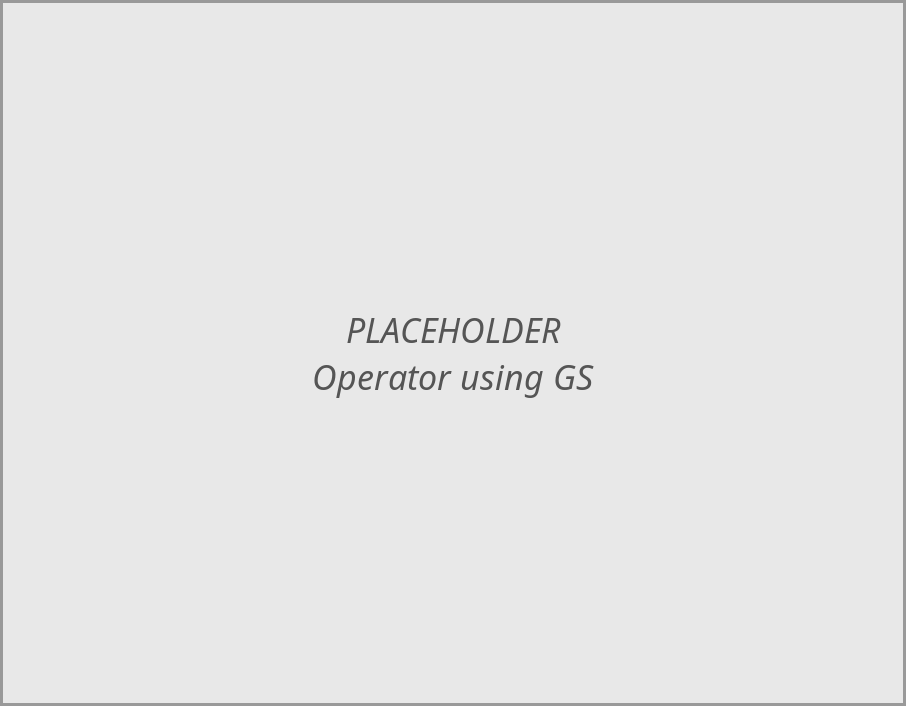
\includegraphics[height=5cm, keepaspectratio]{teams/ground_station/figures/gs_operator.png}
        \caption{Ground station with two operators}
        \label{fig:gs_operators}
    \end{subfigure}
    \hfill
    \begin{subfigure}[c]{0.49\textwidth}
        \centering
        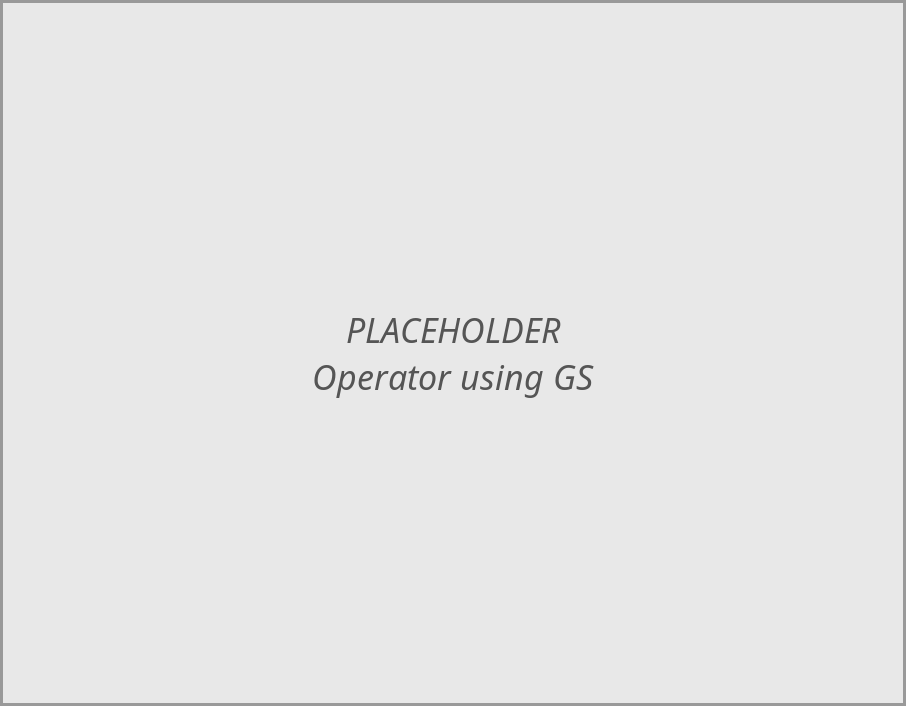
\includegraphics[height=5cm, keepaspectratio]{teams/ground_station/figures/gs_sizes_scheme.png}
        \caption{Ground station scheme with sizes}
        \label{fig:gs_sizes_scheme}
    \end{subfigure}

    \caption{}
\end{figure}
